\section {The arduino}
\begin {frame} {Outline}
    \tableofcontents [current]
\end {frame}

\begin {frame} {The micro controller development board}
    \begin {center}
    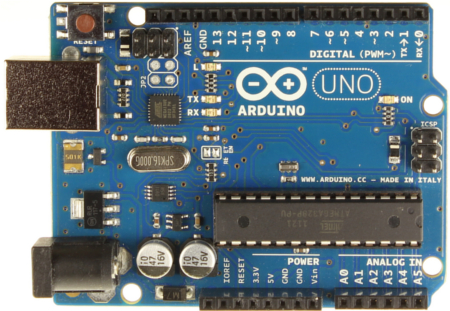
\includegraphics [width=.7\textwidth,keepaspectratio] {img/arduino}
    \end {center}
\end {frame}

\begin {frame} {Why a micro controller development board}
    \begin {itemize}
		\item to sense and control the physical world
		\pause
		\item to develop interactive objects
		\pause
		\item taking inputs from switches or sensors
		\pause
		\item controlling lights, motors, …
		\pause
		\item then do many useful stuff based on that (or not)
    \end {itemize}
\end {frame}

\begin{frame}{Why Arduino ?}
	\begin{itemize}
		\item inexpensive
		\pause
		\item cross-platform
		\pause
		\item simple and don't require electronic skills
		\pause
		\item open source (software and hardware)
	\end{itemize}
\end{frame}

\begin{frame}{The arduino development board}
	Most of the different kinds of arduino are composed by :
	\begin{itemize}
		\item a power connector
		\pause
		\item an USB port (used as a power source and serial port)
		\pause
		\item a reset button
		\pause
		\item some leds (TX RX and pin 13 and power)
		\pause
		\item Ground, 5V and 3.3V pins
		\pause
		\item an ATmega micro controller
		\pause
		\item analog input pins (A0 to A5)
		\pause
		\item some digital pins (0 to 13)
	\end{itemize}
\end{frame}

% we show the different components of the arduino board
\begin{frame}{The micro controller development board}
    \begin{center}
    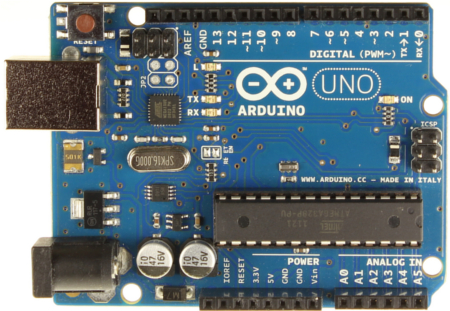
\includegraphics [width=.9\textwidth,keepaspectratio] {img/arduino}
    \end{center}
\end{frame}

% we show the different components of the arduino board
\begin{frame}{And the other arduino boards}
	\begin{itemize}
		\item ARM based
		\item Tiny (specially for IoT)
		\item … or do it yourself (not really difficult)
		% There is no real limit, you just do whatever you can do with the power supplied by arduino
	\end{itemize}
\end{frame}

\begin{frame}{The micro controller development board}
\begin {columns} [c,onlytextwidth]
	\begin {column} [c] {.5\textwidth}
		\begin {center}
			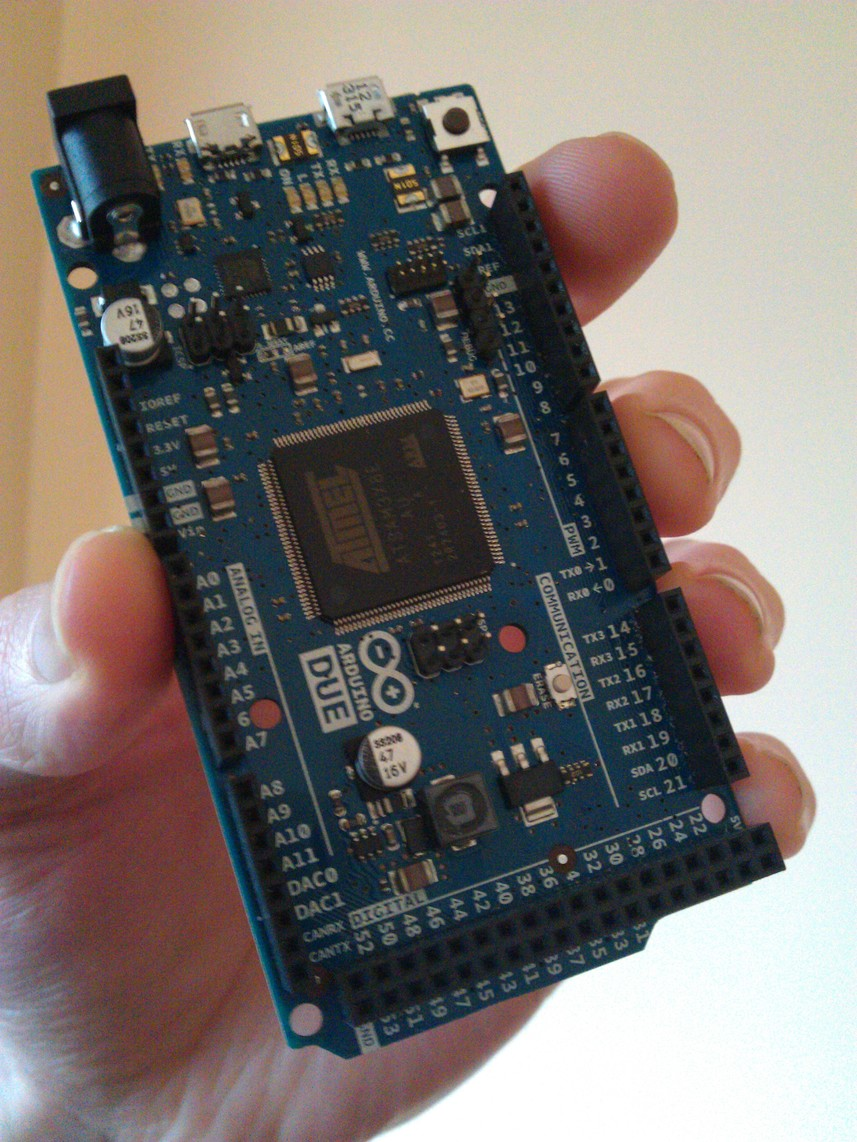
\includegraphics [width=.9\textwidth,keepaspectratio]{img/due}
		\end {center}
	\end {column}
	\pause
	\begin {column} [c] {.5\textwidth}
		\begin {center}
			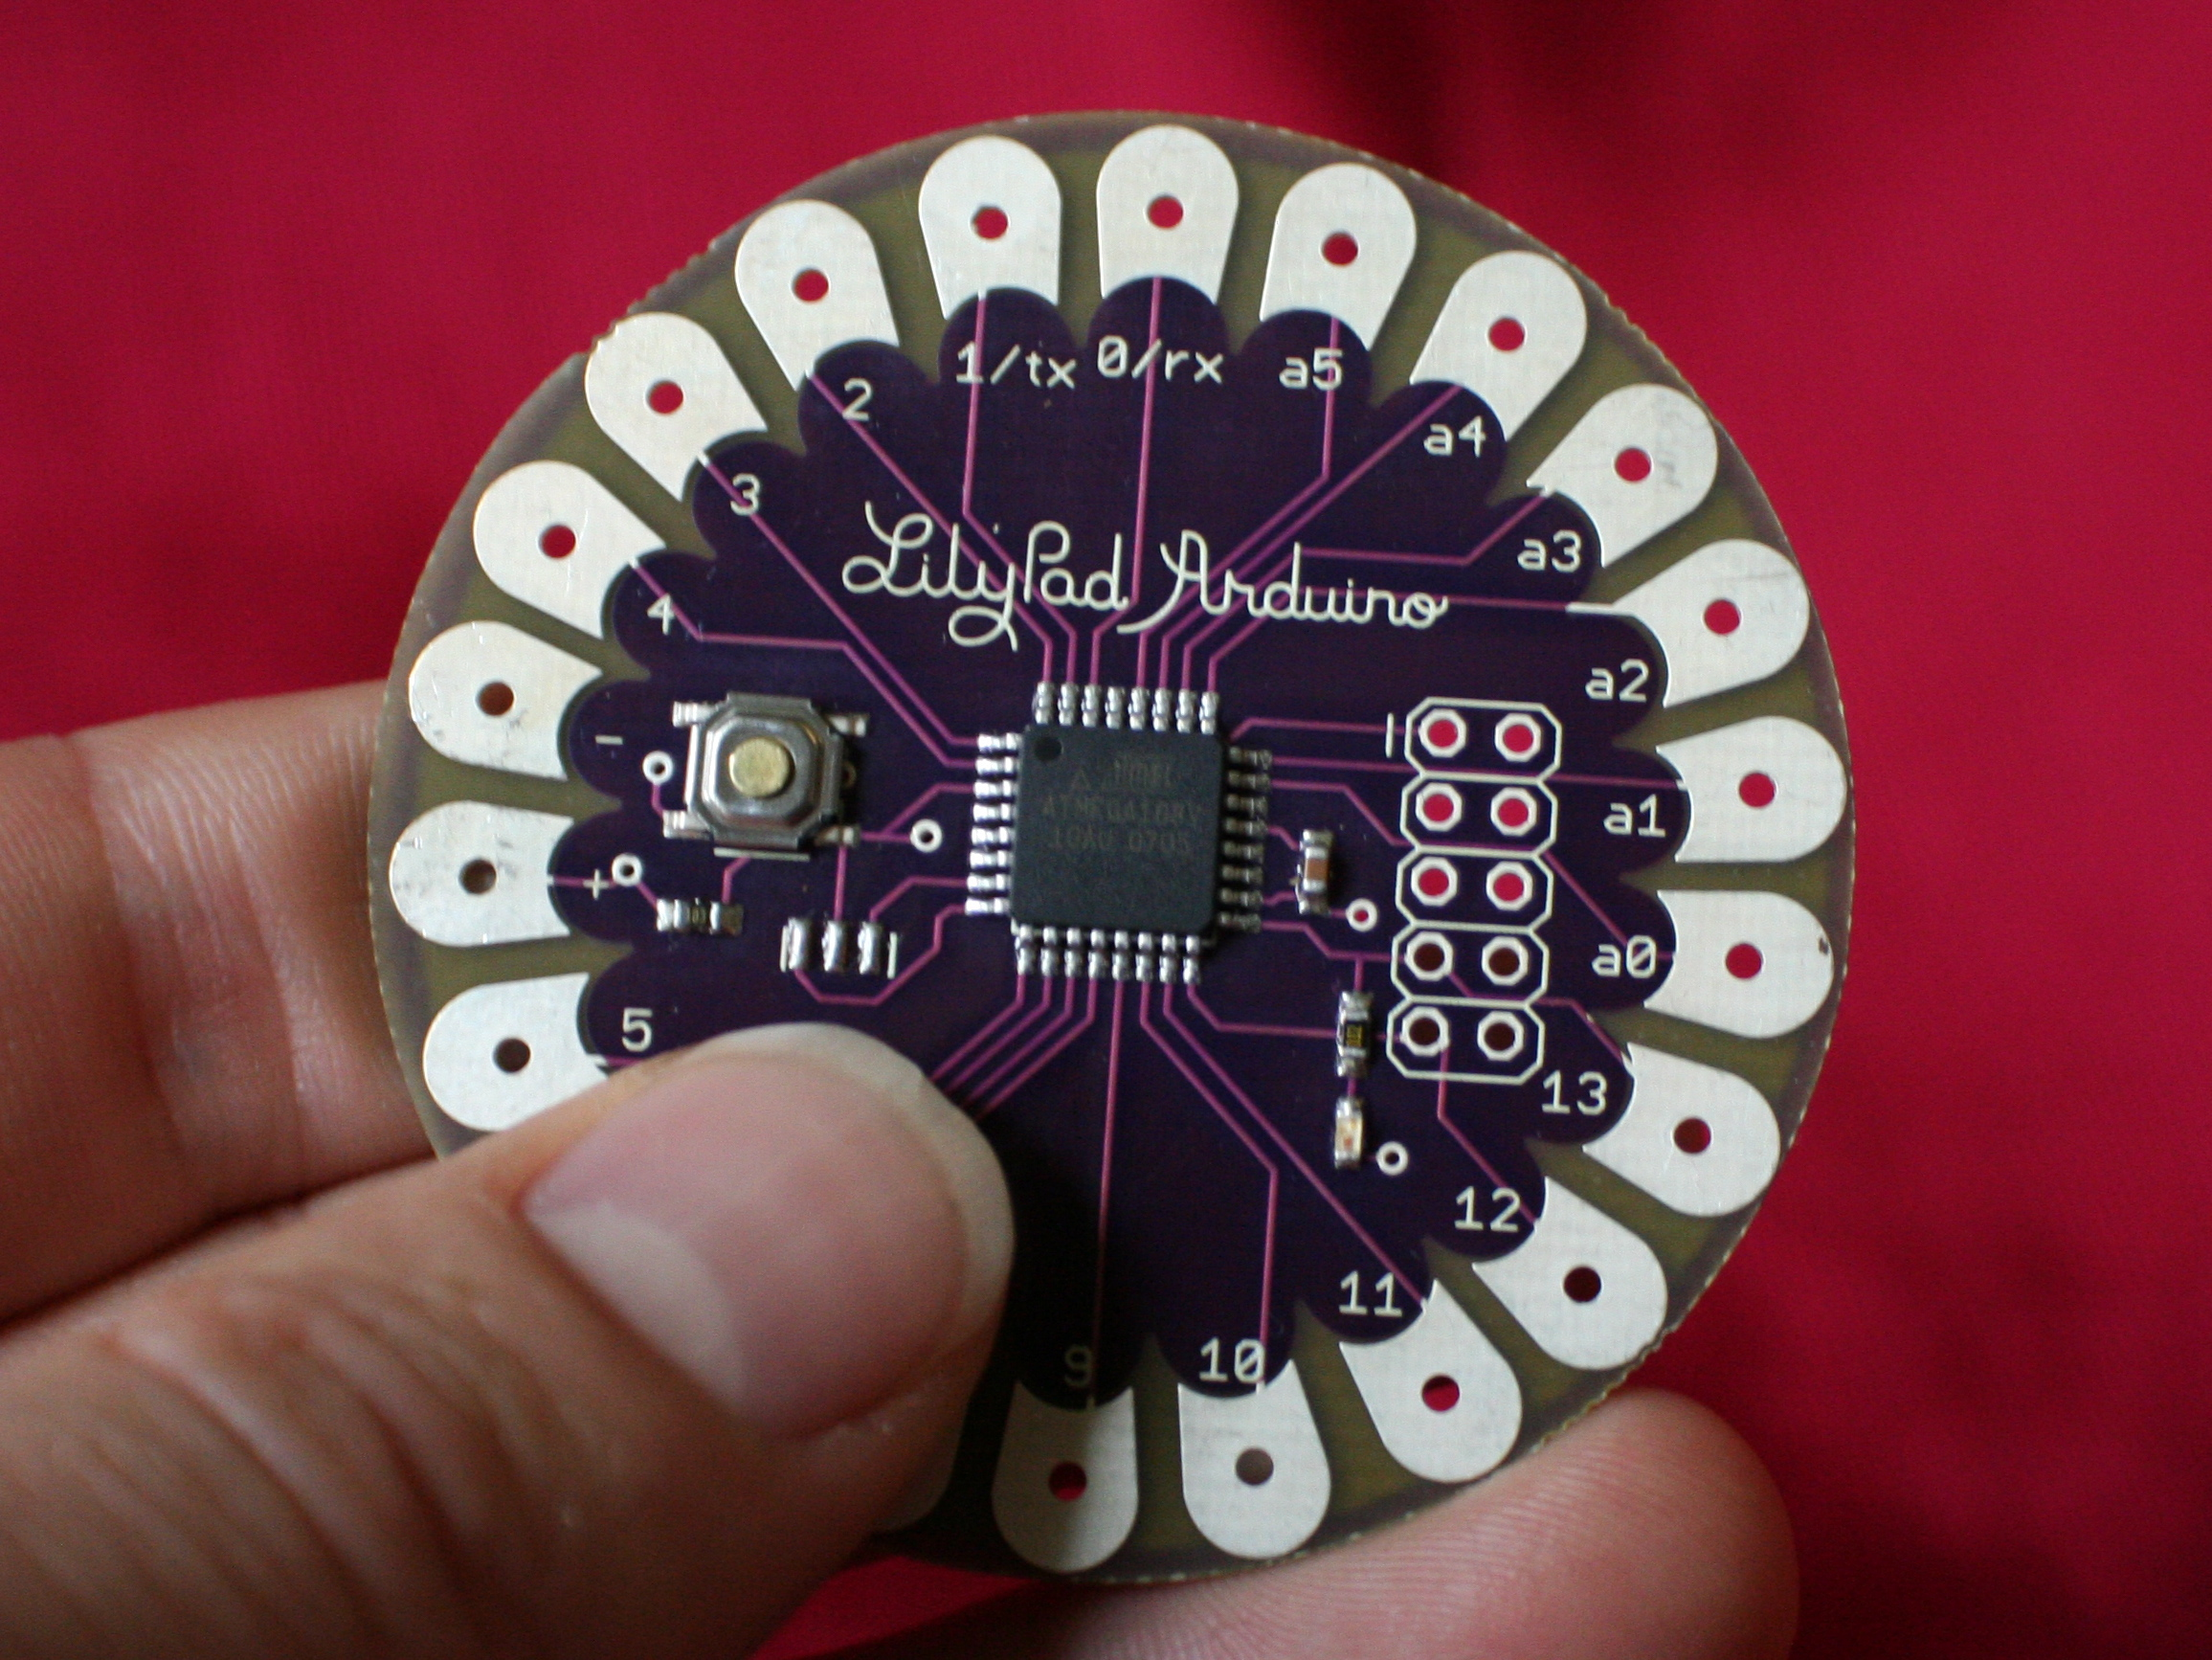
\includegraphics [width=.9\textwidth,keepaspectratio]{img/lilypad}
		\end {center}
	\end {column}
\end {columns}

\end{frame}
